\documentclass[italian,12pt,a4paper,oneside,final]{report}
\usepackage[toc]{appendix}
\usepackage{listings}
\usepackage{graphicx}
\usepackage[utf8]{inputenc}
\usepackage[
backend=biber,
style=numeric,
sorting=none
]{biblatex} %Imports biblatex package
\addbibresource{tickets.bib} %Import the bibliography file
\usepackage[italian]{babel}
\usepackage{csquotes}
\usepackage{hyperref}
\graphicspath{ {images/} }
\lstset{captionpos=b,showspaces=false,basicstyle=\ttfamily,showstringspaces=false,breaklines=true, frame=line}
\renewcommand{\thesection}{\arabic{section}} % remove the \chapter counter from being printed with every \section
\renewcommand{\appendixtocname}{Appendice}
\renewcommand{\appendixpagename}{Appendice}
\hypersetup{
	colorlinks=true,
	linkcolor=,
	urlcolor=blue,
	pdftitle={Marco Giunta - Progetto CS},
	pdfauthor={Marco Giunta},
}

\title{\Large Piattaforma per la distribuzione di\\biglietti gratuiti per eventi\\[0.5em]
	\large Relazione Progetto CS}
\date{Giugno 2025}
\author{
	Marco Giunta\thanks{Marco Giunta 147852 giunta.marco@spes.uniud.it}\\
	Cybersecurity 2024/25, Università degli Studi di Udine}

\begin{document}
\pagenumbering{roman}% To avoid duplicate hyperref links to pages with same page number
% Generate title page
\maketitle
	
% Generate TOCs
\pagenumbering{arabic}
\tableofcontents

\newpage
\section{Introduzione}
Il progetto nasce dall'esigenza di una Segreteria Studenti di un piccolo Ateneo di distribuire ai propri utenti dei biglietti gratuiti per poter assistere a eventi di vario genere (sportivo, culturale, etc).

Attualmente gli utenti di questo Ateneo ricevono via mail un avviso della disponibilità di un certo numero di biglietti per un evento e, se interessati, rispondono via mail alla Segreteria Studenti, la quale, raccolte le adesioni, estrae i nominativi dei vincitori.
Questo metodo di lavoro presenta almeno due criticità:
\begin{itemize}
	\item è possibile che qualche mail di adesione vada persa
	\item è difficile dimostrare la completa casualità nella scelta dei vincitori
\end{itemize}

Con questo progetto si vuole realizzare una piattaforma web per la distribuzione di biglietti gratuiti progettata in modo da assicurare la partecipazione di tutti gli utenti interessati all'evento e garantire la casualità delle estrazioni.

\subsection{Obiettivi del progetto}

Il progetto ha come obiettivo la creazione di una pagina web dove un utente può vedere, senza bisogno di registrazione, la lista degli eventi e, se interessato, può registrarsi e chiedere di partecipare all'estrazione dei biglietti.
Gli eventi vengono inseriti dalla Segreteria Studenti, la quale, dopo aver raccolto le adesioni, procede all'estrazione dei vincitori.
Se l'utente è stato fortunato, troverà all'interno del sito il biglietto per l'evento. 

I dati (eventi, utenti e vincite) sono salvati all'interno di un database MariaDB\footfullcite{mariadb} mentre l'interfaccia web è stata realizzata in PHP.
Per personalizzare lo stile delle pagine html è stata usata la libreria CSS Bootstrap\footfullcite{bootstrap} . 

Per l’installazione e configurazione del piattaforma web è stata utilizzata la tecnologia dei \textit{container}.
\newpage
\section{Architettura logica e fisica}
Per la realizzazione della piattaforma web sono stati utilizzati questi software:

\begin{itemize}
	\item PHP 8.3
	\item Bootstrap 5.3
	\item Bootstrap Icons
	\item MariaDB 11.4
	\item Apache 2.4
\end{itemize}

\subsection{Pagine web}
Le pagine web sono state scritte usando in parte HTML5 e in parte il linguaggio di scripting server-side PHP.
Per ottimizzare la struttura del codice, tutte le funzioni sono state inserite all'interno di un unico file \mbox{(`/includes/functions.php')} per poi essere \textit{incluso} nelle singole pagine. 
Inoltre sono state realizzare due classi, `MyUsers' e `MyEvents', per gestire rispettivamente utenti ed eventi.

Per quanto riguarda la personalizzazione dell'aspetto delle pagine web è stata utilizzata la libreria CSS Bootstrap.
Molto usata in ambito web, questa libreria fornisce componenti già pronti, facilmente personalizzabili.
Anche le icone visualizzate nelle varie pagine fanno parte di pacchetto aggiuntivo messo a disposizione da Bootstrap. 

\subsection{Database}
Tutti i dati gestiti dalla piattaforma (utenti, eventi, prenotazioni e biglietti) sono salvati all'interno di un database MariaDB, un fork open-source di MySQL.
In figura~\ref{fig:schema_db} possiamo vedere lo schema logico del database.

Visto che la piattaforma è stata progettata per funzionare con un numero elevato di utenti e partendo da un database vuoto ci sarebbe voluto troppo tempo per valutare tutte le funzionalità, sono stati inseriti nel database dati di utenti, eventi, e prenotazioni casuali, generati attraverso l’applicazione web Mockaroo\footfullcite{mokaroo}.

\begin{figure}[!h]
	% center image to the page, not to text
	\centerline{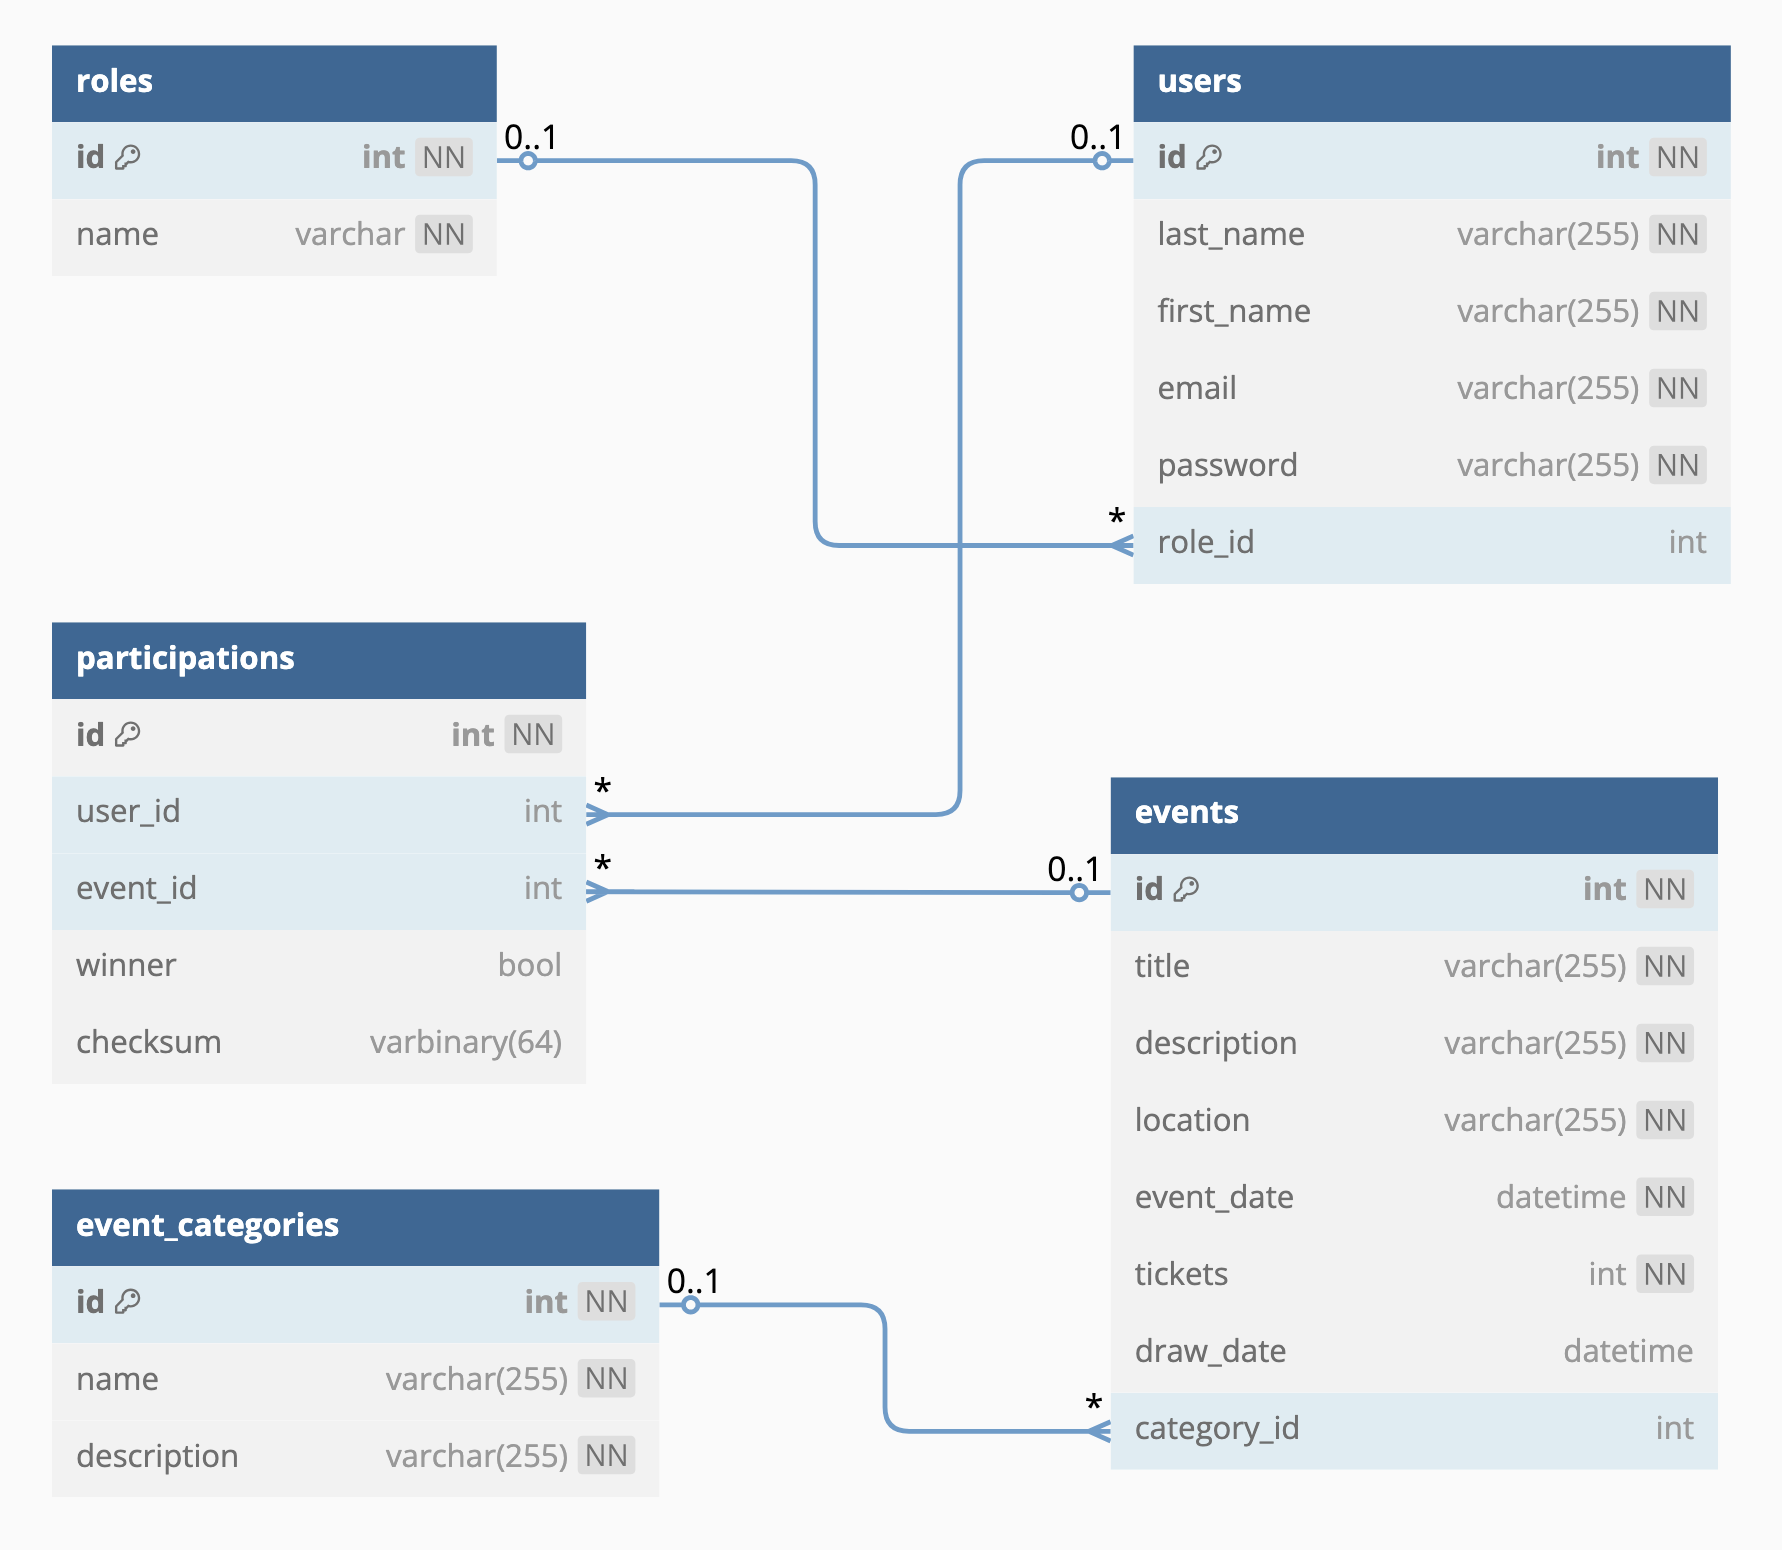
\includegraphics[scale=0.6]{schema_db.png}}
	\caption{Schema logico del database}
	\label{fig:schema_db}
\end{figure}

\subsection{Server web}
Per eseguire gli script PHP e generare le pagine HTML è stato usato il server Web Apache\footfullcite{apache}.

Per aumentare il livello di sicurezza della piattaforma, tutte le pagine sono raggiungibili \textbf{solo} usando il protocollo HTTPS (HyperText Transfer Protocol over Secure Socket Layer ).
Il certificato usato è di tipo \textit{self-sign} ed è necessario aggiungere un eccezione al browser web utilizzato, visto che non è firmato da nessuna CA (Certificate Authority) riconosciuta.
Per forzare l'uso del protocollo HTTPS è stato usato un file `.htaccess', creato all'interno della `DOCUMENT\_ROOT' del server Apache, che effettua un \textit{rewrite} di tutte le richieste.
\hfill \break
\begin{lstlisting}[caption=File .htaccess]
RewriteEngine On
RewriteCond %{HTTPS} off
RewriteRule (.*) https://%{HTTP_HOST}%{REQUEST_URI} [R,L]
\end{lstlisting}

\subsection{Container}
Per la distribuzione e l'installazione del codice della piattaforma web è stata usata la tecnologia dei \textit{container}.

Alcuni dei vantaggi nell'usare i container sono il completo isolamento dal sistema host e la coerenza nella distribuzione delle immagine e del codice.
Ogni container viene eseguito in un area isolata dal resto dei processi presenti sull'host: nel nostro caso, il container Apache comunica con l'esterno \textbf{solo} attraverso le porte di rete 80 e 443.
In caso di compromissione di un container, l'attaccante sarebbe confinato all'interno dello stesso e non riuscirebbe a compromettere l'host o eventuali altri container presenti.
L'immagine di un container è un pacchetto di software eseguibile che include tutto il codice, le dipendenze e gli strumenti necessari per eseguire un’applicazione.
In questo modo, quando si esegue un container su qualunque host, si ha la certezza che venga eseguito senza problemi.

In questo progetto sono stati utilizzati tre diversi container:

\begin{itemize}
	\item mariadb
	\item apache
	\item php
\end{itemize}

\noindent Per distribuire in modo più efficiente l'applicazione è stato usato un \textit{compose file}\footfullcite{docker:compose}.
La configurazione dei software all'interno dei container avviene attraverso l'utilizzo di variabili d'ambiente, specifiche per ogni immagine.
Ad esempio, per configurare i parametri di sessione o il livello di log nel container php, sono state utilizzate queste variabili:
\hfill \break
\begin{lstlisting}[caption=Variabili container php]
PHP_SESSION_USE_ONLY_COOKIES: 'On'
PHP_SESSION_USE_COOKIES: 'On'
PHP_SESSION_REFERER_CHECK: 'localhost'
PHP_SESSION_USE_TRANS_SID: 'Off'
PHP_ERROR_REPORTING: 'Off'
\end{lstlisting}
Mentre per configurare le credenziali di accesso al database dell'immagine di MariaDB, sono state usate queste:
\hfill \break
\begin{lstlisting}[caption=Variabili container mariadb]
MYSQL_ROOT_PASSWORD
MYSQL_DATABASE
MYSQL_USER
MYSQL_PASSWORD
\end{lstlisting}
Per evitare di avere dati sensibili, come la password di accesso al database dell'applicazione, in una variabile d'ambiente accessibile a qualunque utente all'interno del container, e quindi anche ad un possibile attaccante, è stato deciso di utilizzare i \textit{secrets}\footfullcite{docker:secrets}.
In questo modo si riduce anche il rischio di esporre dati sensibili all'esterno dei container, ad esempio nei file di log durante una fase di debug dell'applicazione.

Ogni container può accedere ad una o più directory dell'host: in questo progetto i container apache e php, \textit{montano} la directory `app', dove è contenuto tutto il codice php/html ma, per ragioni di sicurezza, il server Apache non può modificare questi file.
Oltre al codice, il container apache \textit{monta} in sola lettura anche la directory `apache-ssl', contenente il certificato SSL, e il file `apache-conf/vconf-ssl.conf' per la configurazione del virtual host SSL. 

\section{Descrizione del progetto}
La piattaforma web è strutturata per due tipi di utenti, la Segreteria Studenti e gli studenti.
I primi, con privilegi di admin, possono effettuare le seguenti operazioni:

\begin{itemize}
	\item Avere una lista di tutti gli utenti iscritti alla piattaforma
	\item Inserire gli eventi
	\item Controllare i partecipanti al singolo evento
	\item Estrarre i vincitori
	\item Avere una lista di tutti i biglietti assegnati
\end{itemize}
I secondi, invece, possono:
\begin{itemize}
	\item Iscriversi alla piattaforma
	\item Partecipare ad un estrazione
	\item In caso di vittoria, scaricare il biglietto
\end{itemize}
Chiunque può accedere alla lista degli eventi, mentre tutti gli utenti presenti nella piattaforma possono modificare le impostazioni del proprio profilo.
Vediamo in dettaglio alcune funzionalità.

Per iscriversi alla piattaforma è necessario inserire il proprio nome, cognome, email e scegliere una password.
La password dovrà avere certe caratteristiche:
\begin{itemize}
	\item Almeno 8 caratteri
	\item Almeno un numero
	\item Almeno una lettera in maiuscolo
	\item Almeno una lettera in minuscolo
	\item Almeno un carattere speciale (cioè diverso da a-z, A-Z, 0-9 o \_)
\end{itemize}
La password non viene salvata in chiaro nel database, ma viene salvato solo il suo hash di tipo bcrypt, grazie alla funzione PHP `password\_hash'.
Più precisamente, non viene generato un hash a partire dalla sola password, ma viene prima creato un hash hmac-sha256 tra la password in chiaro e una chiave casuale di 32 Bytes (generata durante l'installazione dell'applicazione) e poi viene fatto l'hash bcrypt di questo hash.
In questo modo un eventuale attacco di tipo \textit{brute-force} verso un hash salvato all'interno del database dovrà essere preceduto da un ulteriore \textit{brute-force} verso l'hash hmac.

\noindent In pratica, non basterà fare questo:
\begin{lstlisting}[language=php]
password_verify("a", $hash_del_db)
password_verify("b", $hash_del_db)
...
password_verify("z", $hash_del_db)
password_verify("aa", $hash_del_db)
...
\end{lstlisting}
ma sarà necessario fare questo:
\begin{lstlisting}[language=php]
password_verify(hmac_sha256("a", "a"), $hash_del_db)
password_verify(hmac_sha256("a", "b"), $hash_del_db)
...
\end{lstlisting}
rendendo di fatto impossibile (con le tecnologie attuali) portare a buon fine l'attacco.

Per effettuare il login è necessario inserire la mail e la password scelta in fase di registrazione.
Se le credenziali inserite sono corrette, verrà creata una variabile di sessione PHP con i dati del utente (senza password) e il suo ruolo (admin o user).
Per garantire maggiore sicurezza, in una seconda variabile di sessione viene registrato l'hash del indirizzo IP e dello \textit{user agent} dell'utente che ha effettuato il login.
Questo hash verrà validato in ogni pagina della piattaforma visitata dall'utente.
La validazione avviene grazie alla funzione PHP `hash\_equals', che è immune da attacchi di tipo \textit{Timing attack}.

Nella pagina degli eventi c'è la lista di tutti gli eventi, accessibile a tutti gli utenti, registrati e non.
Dopo il login la piattaforma si comporta in modo diverso, in base al ruolo dell'utente: per gli utenti di tipo admin appare un pulsante che permette la creazione di un nuovo evento.
Per crearne uno nuovo sono necessarie queste informazioni:

\begin{itemize}
	\item Categoria
	\item Titolo
	\item Descrizione
	\item Luogo in cui si svolgerà
	\item Data e ora
	\item Numero di biglietti disponibili
\end{itemize}
Una volta creato l'evento, questo apparirà nella lista degli eventi disponibili e gli utenti registrati potranno, dopo averlo selezionato, premere il pulsante per partecipare all'estrazione dei biglietti.

L'estrazione dei vincitori viene eseguita dagli utenti di tipo admin: quando accedono alla pagina dei dettagli di un evento hanno a disposizione il pulsante `Draw' per far partire l'estrazione.
L'ID degli utenti che hanno chiesto di partecipare all'evento viene inserito in un \textit{array} e, tramite la funzione PHP `random\_int', vengono estratti tanti numeri quanti sono i biglietti a disposizione.
La funzione utilizzata è adatta a tutte le applicazioni, inclusa la generazione di chiavi crittografiche: sfrutta il generatore di numeri casuali del sistema operativo sul quale viene eseguita.
Per evitare azioni di \textit{tampering} sul database, in ogni record relativo alle vincite viene salvato un \textit{checksum}, generato a partire dai dati del vincitore e da una chiave casuale di 32 Bytes che deve essere generata durante l'installazione dell'applicazione.
Questo checksum viene controllato, sempre grazie alla funzione PHP `hash\_equals', ogni volta che si recupera la lista dei vincitori dal database.

Ogni utente registrato può modificare il colore dell'icona del suo avatar, presente nella barra in alto a destra dopo aver fatto il login: questa configurazione viene salvata all'interno di un cookie.
Dato che utenti diversi potrebbero usare lo stesso computer e lo stesso browser web per navigare all'interno della piattaforma, per evitare collisioni il cookie ha un nome diverso per ogni utente: per non esporre informazioni relative all'utente proprietario del cookie, viene utilizzato un hash hmac-sha256 tra i dati dell'utente e la chiave casuale di 32 Bytes vista in precedenza.
Il cookie presenta queste caratteristiche:

\begin{itemize}
	\item ha validità di un anno
	\item vale per tutto il sito
	\item il dominio di utilizzo è solo `localhost'
	\item può essere letto solo via http
	\item funziona solo su connessione sicura https
\end{itemize}

\noindent Per evitare possibili modifiche da parte di un utente malintenzionato, le impostazioni del profilo (in questo caso solo il colore dell'avatar) non sono salvate in chiaro all'interno del cookie, ma vengono criptate usando la funzione PHP `sodium\_crypto\_secretbox', disponibile grazie alla libreria crittografica `sodium'\footfullcite{php:sodium}.
Per criptare o decriptare l'array delle impostazioni dell'utente sono state usate delle funzioni \textit{constant-time}, in grado di resistere ad attacchi di tipo \textit{Timing attack}.

In generale, ogni volta che si chiede all'utente di inserire un dato (dal form di login, alla creazione di un nuovo evento, etc) questo viene sempre validato in base al tipo di dato che ci si aspetta.
Sono state realizzate delle funzioni che testano, attraverso l'utilizzo di \textit{regular expression} o grazie alla funzione PHP `filter\_var', i principali tipi di dati usati nelle piattaforma:

\begin{itemize}
	\item indirizzo email
	\item stringhe di testo
	\item date
	\item numeri interi
	\item colori (secondo il codice colori esadecimale)
\end{itemize}
Prima di essere testati, i dati vengono \textit{sanificati} usando le seguenti funzioni PHP:

\begin{itemize}
	\item trim(): vengono eliminati eventuali spazi, tab o ritorni a capo
	\item stripslashes(): vengono rimossi i caratteri di backslash.
	\item htmlspecialchars(): vengono convertiti i caratteri speciali in entità HTML
\end{itemize}
Inoltre, ogni volta che viene effettuata una query SQL con dati forniti dall'utente, viene sempre fatto il \textit{casting} dei valori, grazie alle funzioni PHP `mysqli\textrightarrow prepare' e `mysqli\textrightarrow bind\_param'.

\section{Conclusioni}
Nel progettare questa piattaforma di distribuzione di biglietti gratuiti per eventi, si è cercato di utilizzare varie tecniche per la realizzazione di applicazioni web sicure: validare tutti i dati di input, per evitare vulnerabilità di tipo Cross-site scripting (XSS) o SQL Injection, utilizzare algoritmi sicuri di hashing, come l’SHA-256, protocolli di comunicazione sicuri, come HTTPS, l'utilizzo dei container, per distribuire ed eseguire il codice, in modo da isolare l'applicazione dal resto dell'infrastruttura.

Per quanto riguarda sviluppi futuri, si potrebbero aggiungere ulteriori funzionalità: gestione completa degli eventi (cancellazione e modifica), cambio password per gli utenti, form di login con captcha o un secondo fattore di autenticazione, annullare la richiesta di partecipazione, etc.
\end{document}